\section{Pay} \label{sec:pay}

\begin{figure}[h!]
  \begin{sequencediagram}
    \newinst{wallet}{\shortstack{Customer wallet \\
      \\ 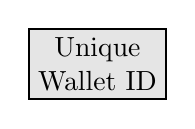
\begin{tikzpicture}
        \node [fill=gray!20,draw=black,thick,align=center] { Unique \\ Wallet ID};
      \end{tikzpicture}
    }}
    \newinst[1]{merchant}{\shortstack{Merchant \\
       \\ \begin{tikzpicture}[shape aspect=.5]
        \tikzset{every node/.style={cylinder,shape border rotate=90, draw,fill=gray!25}}
        \node at (1.5,0) {\shortstack{{{\tiny Database}}}};
       \end{tikzpicture}
    }}
    \newinst[1]{exchange}{\shortstack{Taler (exchange) \\
       \\ \begin{tikzpicture}[shape aspect=.5]
        \tikzset{every node/.style={cylinder,shape border rotate=90, draw,fill=gray!25}}
        \node at (1.5,0) {\shortstack{{{\tiny Database}}}};
       \end{tikzpicture}
    }}
    \newinst[1]{bank}{\shortstack{Merchant bank \\
      \\ 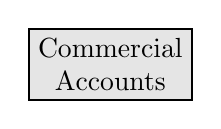
\begin{tikzpicture}
        \node [fill=gray!20,draw=black,thick,align=center] {Commercial \\ Accounts};
      \end{tikzpicture}
    }}
    \postlevel
    \mess[0]{wallet}{Browse catalog}{merchant}
    \mess[0]{merchant}{Commercial offer}{wallet}
    \begin{callself}{wallet}{Review offer}{}
    \end{callself}
    \mess[0]{wallet}{Pay {(Coins)}}{merchant}
    \prelevel
    \mess[0]{merchant}{Deposit {(Coins)}}{exchange}
    \begin{sdblock}{KYC/AML required?}{}
    \begin{callself}{exchange}{Figures~\ref{fig:proc:kyc}, \ref{fig:proc:aml}}{}
    \end{callself}
    \end{sdblock}
    \begin{sdblock}{Acceptable account?}{}
    \mess[0]{exchange}{{Refuse deposit}}{merchant}
    \prelevel
    \mess[0]{merchant}{{Fail purchase}}{wallet}
    \end{sdblock}
    \mess[0]{exchange}{{Confirm deposit}}{merchant}
    \prelevel
    \mess[0]{merchant}{Fulfill order}{wallet}
    \begin{callself}{exchange}{Aggregate transactions}{}
    \end{callself}
    \begin{sdblock}{KYC/AML required?}{}
    \begin{callself}{exchange}{Figures~\ref{fig:proc:kyc}, \ref{fig:proc:aml}}{}
    \end{callself}
    \end{sdblock}
    \mess[0]{exchange}{{Initiate transfer}}{bank}
  \end{sequencediagram}
  \caption{Payments from a customer to merchant result in
    depositing coins at the Taler exchange (payment service provider)
    which then credits the merchant's bank account.
    The KYC/AML checks are described in Section~\ref{sec:kyc:deposit}}
  \label{fig:int:pay}
\end{figure}

{\bf Internal note:} The exchange refusing a deposit immediately based on
unaccaptable merchant accounts can depend both on the target account
(e.g. wire method not supported) or on the legitimization state of the
merchant's target account (including lack of KYC authorization wire
transfer, failure to accept terms of service, failure to provide KYC
data, or some kind of AML/KYC rule being violated).  However, in general
the merchant backend will know if it has performed some mandatory sign-up
process and can thus avoid the entire situation by only offering exchanges
where the merchant is in good standing in its contracts.  The central
bug for supporting this in the merchant is \#9052.
